\documentclass{article}
\usepackage[margin = 2.54cm]{geometry} % set margin to traditional doc

%packages
\usepackage{graphicx} % Required for inserting images
\usepackage[most]{tcolorbox} %for creating environments
\usepackage{amsmath}
\usepackage{amssymb}
\usepackage{mathtools}
\usepackage{verbatim}
\usepackage[utf8]{inputenc}
\usepackage[dvipsnames]{xcolor} %for importing multiple colors
\usepackage{hyperref} %for creating links to different sections

\linespread{1.2} %controlling line spread

%define colors i like
\definecolor{myTeal}{RGB}{0,128,128}
\definecolor{myGreen}{RGB}{34,170,34}
\definecolor{mySapphire}{RGB}{15,82,186}
\definecolor{myEmerald}{RGB}{50.4, 130, 90}

%create math environments, can add [section] or [subsection] to add index counter based on sections/subsections
\newtheorem{define}{Definition}
\newtheorem{prop}{Proposition}
\newtheorem{thm}{Theorem}
\newtheorem{question}{Question}
\newtheorem{lemma}{Lemma}

%setup colored box environment for each math env above
\tcolorboxenvironment{define}{
    enhanced, colframe=myTeal!50!teal, colback=myTeal!10,
    arc=5mm, lower separated=false, fonttitle=\bfseries, breakable
}
\tcolorboxenvironment{prop}{
    enhanced, colframe=myGreen!50!black, colback=myGreen!15,
    arc=5mm, lower separated=false, fonttitle=\bfseries, breakable
}
\tcolorboxenvironment{thm}{
    enhanced, colframe=mySapphire!50!mySapphire, colback=mySapphire!15,
    arc=5mm, lower separated=false, fonttitle=\bfseries, breakable
}
\tcolorboxenvironment{question}{
    enhanced, colframe=blue!50!black, colback=blue!10,
    arc=5mm, lower separated=false, fonttitle=\bfseries, breakable
}
\tcolorboxenvironment{lemma}{
    enhanced, colframe=myEmerald!50!myEmerald, colback=myEmerald!10,
    arc=5mm, lower separated=false, fonttitle=\bfseries, breakable
}

%setup hyperlink within pdf
\hypersetup{
    colorlinks=true,
    linkcolor=blue,
    filecolor=magenta,      
    urlcolor=cyan,
    pdftitle={Overleaf Example},
    pdfpagemode=FullScreen,
}

%common command (add to template)
%general
\newcommand{\FF}{\mathbb{F}}
\newcommand{\NN}{\mathbb{N}}
\newcommand{\ZZ}{\mathbb{Z}}
\newcommand{\QQ}{\mathbb{Q}}
\newcommand{\RR}{\mathbb{R}}
\newcommand{\CC}{\mathbb{C}}

\newcommand{\Id}{\textmd{Id}} %identity
\newcommand{\lcm}{\textmd{lcm}}
\DeclarePairedDelimiter{\abs}{\lvert}{\rvert}
\DeclarePairedDelimiter{\norm}{\lVert}{\rVert}
\DeclarePairedDelimiter{\paran}{(}{)}%paranthesis
\DeclarePairedDelimiter{\bracket}{\langle}{\rangle}

%algebra
\newcommand{\Gal}{\textmd{Gal}}
\newcommand{\Aut}{\textmd{Aut}}
\newcommand{\End}{\textmd{End}}
\newcommand{\Coker}{\textmd{Coker}}
\newcommand{\Hom}{\textmd{Hom}}
\newcommand{\Nil}{\textmd{Nil}}
\newcommand{\Char}{\textmd{char}}
    %linear algebra basis
    \newcommand{\be}{\textmd{e}}

%analysis
\newcommand{\Vol}{\textmd{Vol}}

%complex
\newcommand{\Real}{\textmd{Re}}
\newcommand{\Imag}{\textmd{Im}} %can also be used for Image
\newcommand{\Res}{\textmd{Res}}

%lie algebra
\newcommand{\gl}{\mathfrak{gl}}

%physics
\newcommand{\br}{\textbf{r}} %position
\newcommand{\bv}{\textbf{v}} %velocity
\newcommand{\ba}{\textbf{a}} %cceleration
\newcommand{\bF}{\textbf{F}} %force
\newcommand{\bP}{\textbf{P}} %momentum
\newcommand{\bL}{\textbf{L}} %angular momentum
\newcommand{\bN}{\textbf{N}} %torque
\newcommand{\bw}{\textbf{w}} %angular velocity
\newcommand{\bzero}{\textbf{0}}

\title{Phys 103 HW3}
\author{Zih-Yu Hsieh}

\begin{document}
\maketitle

\section*{1}
\begin{question}\label{q1}
    A cylindrical pole is inserted into a frozen lake to the pole stands vertically. One end of a rope is attached to a point on the surface of the pole near where it enters the ice, and the rope is then laid out in a straight line on the surface. An ice skater with initial velocity $\bv_0$ approaches the opposite end of the rope, moving perpendicular to the rope. As she reaches the rope she grabs it and holds on, and the rope then winds up around the pole.
    \begin{itemize}
        \item[(a)] Has there been any change in her kinetic energy? If so, identify what positive or negative work has been done on her, and by what source.
        \item[(b)] Has there been any change in her angular momentum? If so, identify the source of the torque done upon her.
        \item[(c)] When the rope is half wound up, what is her speed, assuming there is no friction between the rope or herself and the ice?
    \end{itemize}
\end{question}

\textbf{Pf:}

Overall, if the pole is modeled with radius $r=0$, it will eventually be nonsensical because the rope is assumed to be decreasing in length when winding up around the pole (if $r=0$, the rope length wouldn't decrease). So, here we'll assume the pole has radius $r>0$ that can't be disregarded.

Also, because the system is on a frozen lake, one can assume that the friction force in general is small, hence we'll ignore friction for easier calculation.

\begin{figure}[h!]
    \begin{center}
        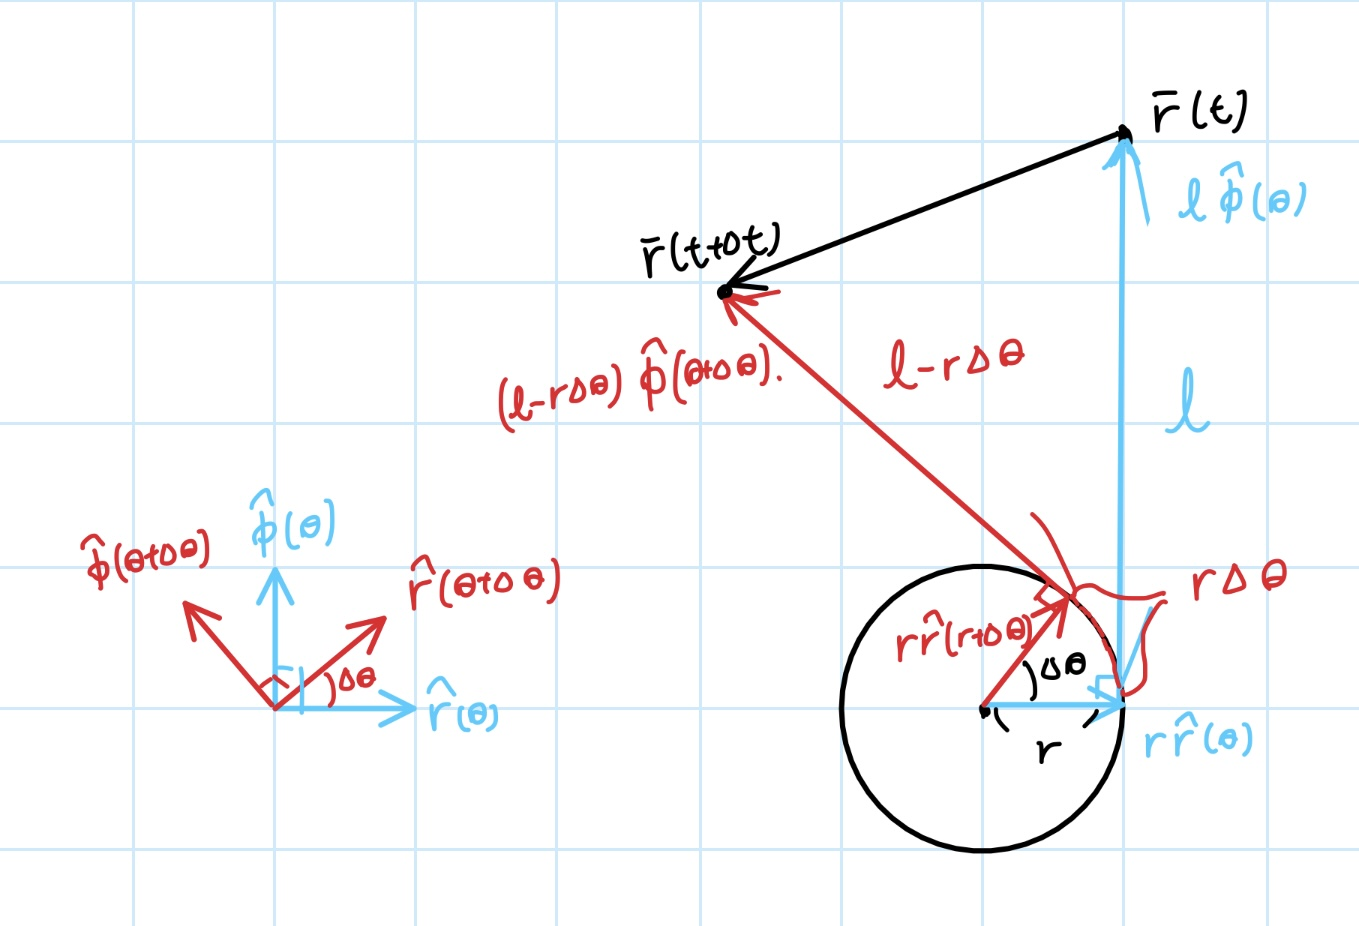
\includegraphics[width=71.5mm]{phys103_q1a.jpg}
        \caption{Polar Coordinates used for Derivation}
    \end{center}
\end{figure}

Before starting, I want to analyze the relationships between the force applied on the skater, and the path the skater took: In general, if the rope is always taut, can assume it's always tangential to the surface of the pole (i.e. it is a tangent line to the circle of the pole, when viewed from above). 

Which, WLOG assume the skater is going in counterclockwise motion, suppose at time $t_0$ the angle of the contact point is $\theta$ (with the rope's length $l>0$), and after time period $\Delta t>0$, the change in angle is $\Delta \theta$ (while the rope maintains with positive length). Then, based on the graph, we get the following:
\begin{align}
    t=t_0 \implies \begin{cases}
        \textmd{rope's contact point} &= r\hat{r}(\theta)\\
        \textmd{displacement of rope} &= l\hat{\phi}(\theta)\\
        \textmd{skater position }\br(t_0) &= r\hat{r}(\theta)+l\hat{\phi}(\theta)
    \end{cases}
\end{align}
\begin{align}
    t=t_0+\Delta t \implies \begin{cases}
        \textmd{rope's contact point} &= r\hat{r}(\theta+\Delta\theta)\\
        \textmd{displacement of rope} &= (l-r\Delta \theta)\hat{\phi}(\theta+\Delta\theta)\\
        \textmd{skater position }\br(t_0+\Delta t) &= r\hat{r}(\theta+\Delta\theta) + (l-r\Delta\theta)\hat{\phi}(\theta+\Delta\theta)
    \end{cases}
\end{align}
(Note: after wrapping around the pole with angle $\Delta\theta$, the decreased rope length is the arc length $r\Delta\theta$, that's why after time becomes $t=t_0+\Delta t$, the length of the rope is $(l-r\Delta\theta)$).

Then, if taken the limit as $\Delta t\rightarrow 0$, we get the following for velocity:
\begin{align}
    \bv(t_0)&=\lim_{\Delta t\rightarrow 0}\frac{\br(t_0+\Delta t)-\br(t_0)}{\Delta t}=\lim_{\Delta t\rightarrow 0}\frac{\Delta\theta}{\Delta t}\cdot\frac{\br(t_0+\Delta t)-\br(t_0)}{\Delta\theta}\\
    &= \lim_{\Delta t\rightarrow 0}\frac{\Delta\theta}{\Delta t}\cdot\frac{1}{\Delta \theta}\paran*{\paran*{r\hat{r}(\theta+\Delta\theta)+(l-r\Delta\theta)\hat{\phi}(\theta+\Delta\theta)} - \paran*{r\hat{r}(\theta)+l\hat{\phi}(\theta)}}\\
    &= \lim_{\Delta t\rightarrow 0}\frac{\Delta\theta}{\Delta t}\cdot\paran*{
        r\frac{\hat{r}(\theta+\Delta\theta)-\hat{r}(\theta)}{\Delta\theta} + \frac{(l-r\Delta\theta)\hat{\phi}(\theta+\Delta\theta)-l\hat{\phi}(\theta)}{\Delta\theta}
    }\\
    &= \lim_{\Delta t\rightarrow 0}\frac{\Delta\theta}{\Delta t}\cdot\paran*{r\frac{\hat{r}(\theta+\Delta\theta)-\hat{r}(\theta)}{\Delta\theta} - r\hat{\phi}(\theta+\Delta\theta)+ l\frac{\hat{\phi}(\theta+\Delta\theta)-\hat{\phi}(\theta)}{\Delta\theta}}\\
    &= \frac{d\theta}{dt}\cdot \paran*{r\frac{d\hat{r}}{d\theta} - r\hat{\phi}+l\frac{d\hat{\phi}}{d\theta}}\bigg|_{t = t_0} = \frac{d\theta}{dt}\cdot\paran*{r\hat{\phi} -r\hat{\phi}-l\hat{r}} = -l\frac{d\theta}{dt}\hat{r}(\theta)
\end{align}
This shows that at any time $t$, the velocity $\bv$ is always in radial direction $\hat{r}$, while based on the graph, since the rope is always tangential to the pole (with displacement in $\hat{\phi}$ direction), the tension force on the skater $\bF_T = -F_T\hat{\phi}$. Which, we get the following graph as relation:

\begin{figure}[h!]
    \begin{center}
        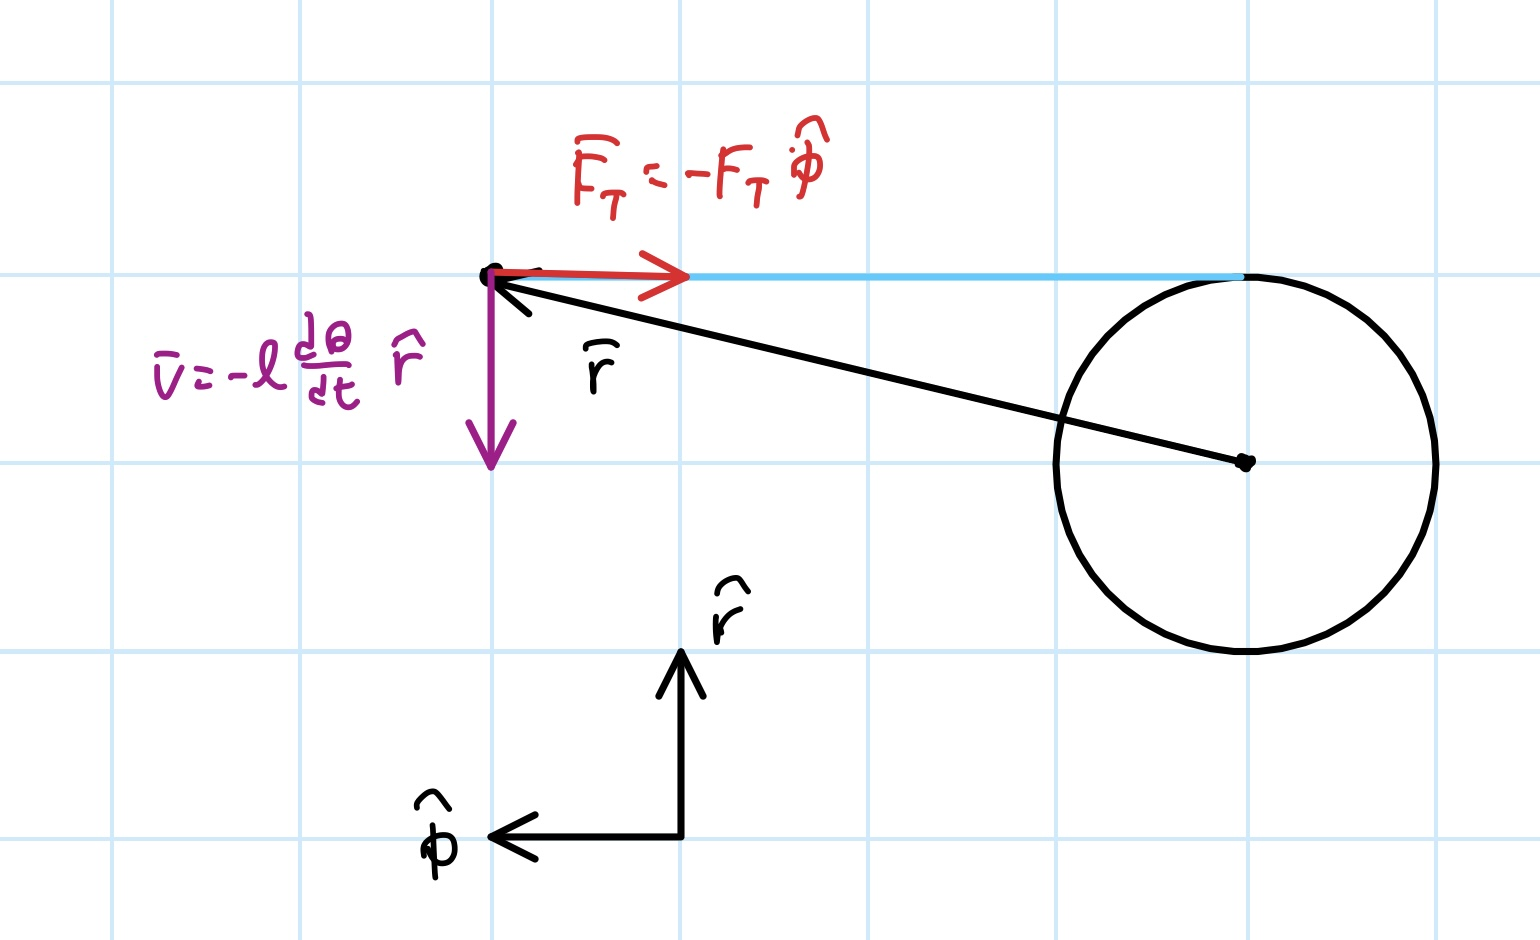
\includegraphics[width=71mm]{phys103_q1a2.jpg}
        \caption{Relations of each vector components}
    \end{center}
\end{figure}

\subsection*{(a)}
To analyze the change in kinetic energy, consider the following: At each time $t$, and the rope's contact point's angle with the pole being $\theta$, the velocity of the skater is $\bv(t)=-l\frac{d\theta}{dt}\hat{r}$, while the only force applied on the skater is the tension force $\bF_T(t) = -F_T(t)\hat{\phi}$ (where $F_T(t)>0$ for the skater to stay contact with the rope), hence the net power on the skater, $P(t) = \bF_T(t)\cdot \bv(t) = 0$ (since the force and velocity is always orthogonal). Because power $P=\frac{dE}{dt}$ (where $E$ is the energy), this shows that the mechanical energy is constant under this model. And, because can assume there's no potential energy in this scenario (no conservative force involved, etc.), then the total mechanical energy can be viewed as the kinetic energy only. Hence, the kinetic energy of the skater is not changing.

\subsection*{(b)}
To analyze the change in angular momentum, consider the following: At each time $t$, with the rope's length $l>0$, and the rope contacting with the pole at angle $\theta$, the position of the skater is $\br(t)=r\hat{r}+l\hat{\phi}$, while the only source of force is the tension force $\bF_T(t)=-F_T(t)\hat{\phi}$ (described in part (a) also). Which, in the model we assume the radius of the pole $r>0$, then with the component $r\hat{r}\neq\bzero$ in $\br(t)$, we see that $\br(t)$ and the force $\bF_T(t)$ are not parallel (since $\bF_T$ is in $\hat{\phi}$ direction, orthogonal to $\hat{r}$). Hence, the net torque $\bN(t) = \br(t)\times \bF_T(t)\neq \bzero$, showing that some nonzero torque is applied on the skater. Hence, the angular momentum is not constant, and the source of the torque is from the tension force of the rope.

\subsection*{(c)}
Using conservation of energy described in part (a), with the skater's mass $m>0$, her initial kinetic energy $K_0 = \frac{1}{2}mv_0^2$ (where $v_0=\|\bv_0\|$, $\bv_0$ is the initial velocity). Which, at the final point with speed $v_f$, we must have $\frac{1}{2}mv_f^2 = K_f = K_0 = \frac{1}{2}mv_0^2$. With the mass $m>0$ not changing, we must have $v_f^2=v_0^2$; and with both $v_f,v_0\geq 0$ (assume they're speed), then $v_f=v_0$.

\break

\section*{2 (Insert image)}
\begin{question}\label{q2}
    Consider an equilateral triangle of mass $M$, side length $L$, and uniform density. Let's choose coordinates so that the origin is at the center of mass, the triangle (at least initially) lies in the $xy$ plane, and one of the vertices of the triangle (at least initially) is on the positive $x$-axis.
    \begin{itemize}
        \item[(a)] Calculate the inertia tensor of the triangle. To be clear, for this and all later parts you should give answers in the lab frame.
        \item[(b)] Suppose we give the triangle angular speed $w_0$ around the $z$ axis. What is the initial angular momentum (magnitude and direction)? Is the inertia tensor constant in time? Give a qualitative explanation for why and how the inertia tensor and angular velocity do or do not change.
        \item[(c)] Suppose we give the triangle initial angular speed $w_0$ around the $x$-axis. What is the angular momentum (magnitude and direction)? Is the inertia tensor constant in time? Calculate the initial angular acceleration. Is the angular velocity constant in time? Give a qualitative explanation for why and how the inertia tensor and angular velocity do or do not change.
        \item[(d)] Suppose we give the triangle angular velocity $(w_0/\sqrt{2},0,w_0/\sqrt{2})$, i.e., around an axis in between the $x$ and $z$ axes. (Suggestion: use Rotation Matrix function in Mathematica, or other programming languages). What is the initial angular momentum (magnitude and direction)? Is the inertia tensor constant in tiem? Calculate the initial angular acceleration. Is the angular velocity constant in time? Give a qualitative explanation for why and how the inertia tensor and angular velocity do or do not change. 
    \end{itemize}
\end{question}

\textbf{Pf:}

\begin{figure}[h!]
    \begin{center}
        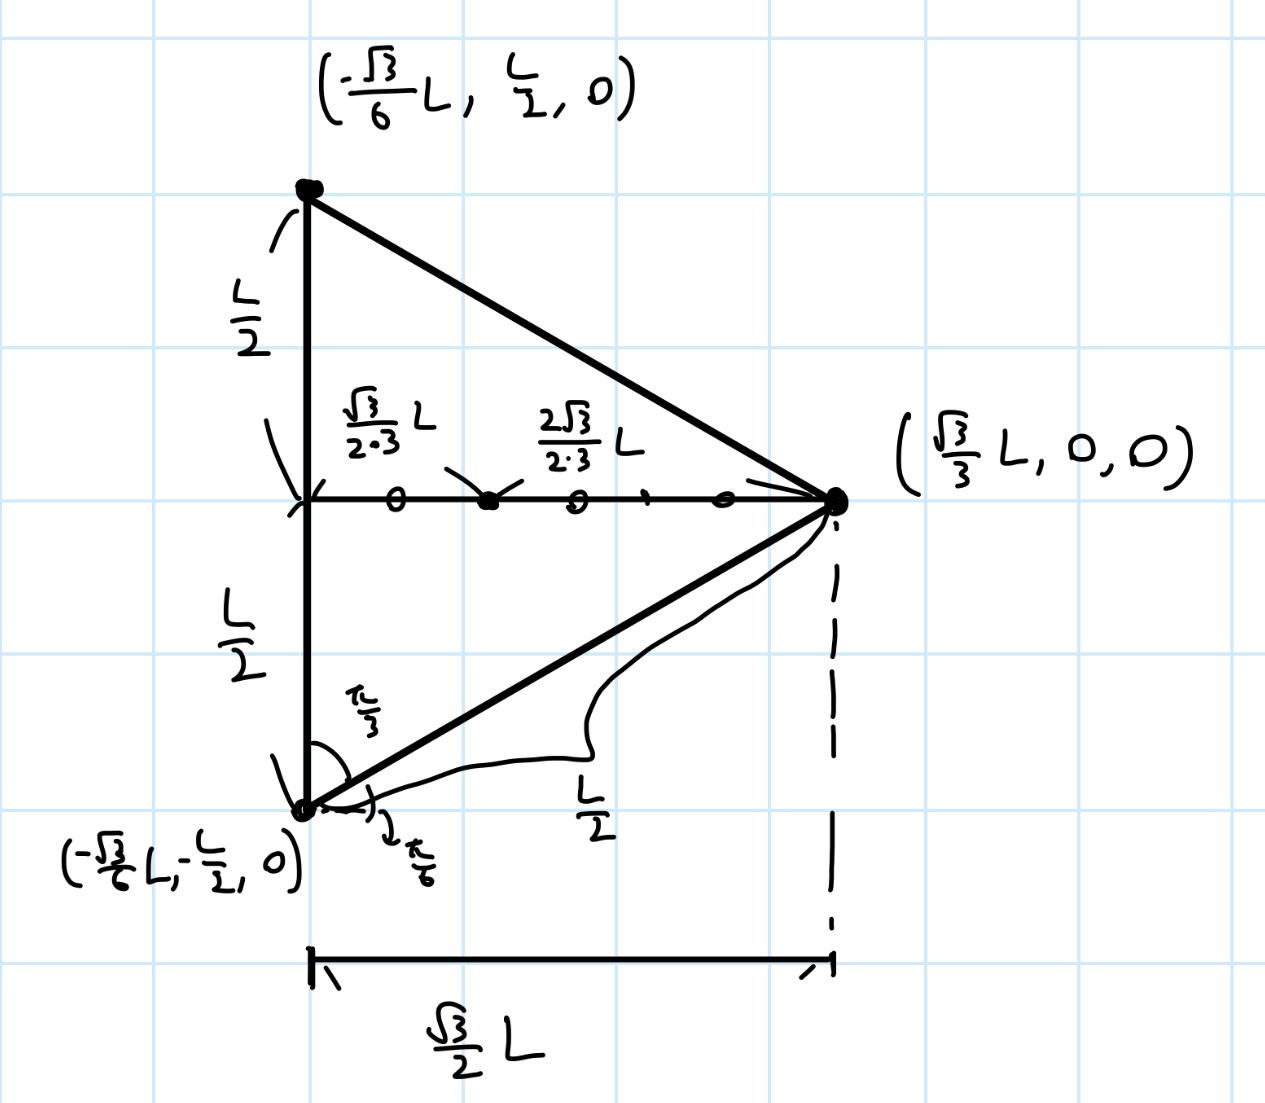
\includegraphics[width=70mm]{phys103_q2.jpg}
        \caption{The relation of Equilateral Triangle with sidelength $L$}
    \end{center}
\end{figure}

\subsection*{(a)}
Given the picture, we got the bound of the integration given as $x\in [-\frac{\sqrt{3}}{6}L, \frac{\sqrt{3}}{3}L]$, and $\frac{\sqrt{3}}{3}x-\frac{1}{3}L\leq y\leq -\frac{\sqrt{3}}{3}x+\frac{1}{3}L$. Now, to calculate the actual inertia tensor,  the height cannot be assumed to be $0$ directly, we'll take the height $z\in [-\epsilon,\epsilon]$ for $\epsilon>0$, and at the end take the limit $\epsilon\rightarrow 0$. 

Which, with side length $L$, the equilateral triangle has base area $A=\frac{\sqrt{3}}{4}L^2$, and with height $2\epsilon$ based on the chosen range of $z$, the total volume is $V=\frac{\sqrt{3}}{2}L^2\epsilon$, showing that the density $\rho = \frac{M}{V}=\frac{2\sqrt{3}M}{3L^2\epsilon}$. Then, taken the inertia tensor, we get:
\begin{align}
    I(\epsilon) &= \int_{z=-\epsilon}^{\epsilon}\int_{x=-\frac{\sqrt{3}}{6}L}^{\frac{\sqrt{3}}{3}L}\int_{y=\frac{\sqrt{3}}{3}x-\frac{1}{3}L}^{-\frac{\sqrt{3}}{3}x+\frac{1}{3}L} \begin{pmatrix}
        y^2+z^2 & -xy & -xz\\
        -xy & x^2+z^2 & -yz\\
        -xz & -yz & x^2+y^2
    \end{pmatrix}\rho\ dy\ dx\ dz
\end{align}
Which, notice that the integration bound of $x,y,z$ are all symmetric (from $-a$ to $a$ when fixing $(x,y,z)$), so when viewed as single-variable functions, $xy,yz,xz$ would all be odd functions, then the integration bound would provide $0$ regardless of the order of integration (for $xy$ and $yz$, since it's an odd function of $y$, the integration of $y$ generate $0$; then for $xz$, since integrating with respect to $y$ then $x$ generates a constant, so it remains as an odd function of $z$, hence the final integration with respect to $z$ provides $0$). 

So, it remains to check the diagonal entries. Doing the integrals, we get:
\begin{align}
    Y&:=\int_{z=-\epsilon}^{\epsilon}\int_{x=-\frac{\sqrt{3}}{6}L}^{\frac{\sqrt{3}}{3}L}\int_{y=\frac{\sqrt{3}}{3}x-\frac{1}{3}L}^{-\frac{\sqrt{3}}{3}x+\frac{1}{3}L}y^2dy\ dx\ dz = -\frac{2}{3}\int_{z=-\epsilon}^{\epsilon}\int_{x=-\frac{\sqrt{3}}{6}L}^{\frac{\sqrt{3}}{3}L}\paran*{\frac{\sqrt{3}}{3}x-\frac{1}{3}L}^3 dx\ dz\\
    &= -\frac{2}{3}\cdot 2\epsilon\cdot \frac{\sqrt{3}}{4}\paran*{\frac{\sqrt{3}}{3}x-\frac{1}{3}L}^4\bigg|_{-\frac{\sqrt{3}}{6}L}^{\frac{\sqrt{3}}{3}L}= -\frac{\sqrt{3}\epsilon}{3}\paran*{0-\frac{L^4}{16}} = \frac{\sqrt{3}L^4\epsilon}{48}
\end{align}
\begin{align}
    Z&:=\int_{z=-\epsilon}^{\epsilon}\int_{x=-\frac{\sqrt{3}}{6}L}^{\frac{\sqrt{3}}{3}L}\int_{y=\frac{\sqrt{3}}{3}x-\frac{1}{3}L}^{-\frac{\sqrt{3}}{3}x+\frac{1}{3}L}z^2 dy\ dx\ dz= \frac{2}{3}\epsilon^3\int_{x=-\frac{\sqrt{3}}{6}L}^{\frac{\sqrt{3}}{3}L}\paran*{-\frac{2\sqrt{3}}{3}x+\frac{2}{3}L}dx\\
    &= -\frac{3}{2\sqrt{3}}\cdot \frac{2\epsilon^3}{3}\cdot\frac{1}{2}\paran*{-\frac{2\sqrt{3}}{3}x+\frac{2}{3}L}^2\bigg|_{-\frac{\sqrt{3}}{6}L}^{\frac{\sqrt{3}}{3}L}= -\frac{\sqrt{3}\epsilon^3}{6}\paran*{0-L^2} = \frac{\sqrt{3}L^2\epsilon^3}{6}
\end{align}
\begin{align}
    X&:= \int_{z=-\epsilon}^{\epsilon}\int_{x=-\frac{\sqrt{3}}{6}L}^{\frac{\sqrt{3}}{3}L}\int_{y=\frac{\sqrt{3}}{3}x-\frac{1}{3}L}^{-\frac{\sqrt{3}}{3}x+\frac{1}{3}L}x^2 dy\ dx\ dz= 2\epsilon \int_{x=-\frac{\sqrt{3}}{6}L}^{\frac{\sqrt{3}}{3}L}-2x^2\paran*{\frac{\sqrt{3}}{3}x-\frac{1}{3}L}dx\\
    &= 2\epsilon\paran*{
        -\frac{2\sqrt{3}}{3}\int_{-\frac{\sqrt{3}}{6}L}^{\frac{\sqrt{3}}{3}L}x^3dx + \frac{2L}{3}\int_{-\frac{\sqrt{3}}{6}L}^{\frac{\sqrt{3}}{3}L}x^2dx
    }= 2\epsilon\paran*{
        -\frac{5\sqrt{3}}{288}L^4+\frac{\sqrt{3}L^4}{36}
    }=\frac{\sqrt{3}L^4\epsilon}{48}
\end{align}
With $X=Y$, plug the results into $I$ (and with $\rho$ being a constant), we get:
\begin{align}
    I(\epsilon)=\rho\begin{pmatrix}
        Y+Z&0&0\\
        0&X+Z&0\\
        0&0&X+Y
    \end{pmatrix} = \rho \begin{pmatrix}
        X+Z&0&0\\
        0&X+Z&0\\
        0&0&2X
    \end{pmatrix}
\end{align}
Then, with the above expression of $X,Z,\rho$, we get the following limits:
\begin{align}
    \lim_{\epsilon\rightarrow 0}\rho X = \lim_{\epsilon\rightarrow 0}\frac{2\sqrt{3}M}{3L^2\epsilon}\cdot\frac{\sqrt{3}L^4\epsilon}{48} = \frac{ML^2}{24}, \quad \lim_{\epsilon\rightarrow 0}\rho Z = \lim_{\epsilon\rightarrow 0}\frac{2\sqrt{3}M}{3L^2\epsilon}\cdot\frac{\sqrt{3}L^2\epsilon^3}{6}=0
\end{align}
Hence, the actual inertia tensor is:
\begin{align}
    I = \lim_{\epsilon\rightarrow 0}I(\epsilon) = \frac{ML^2}{24}\begin{pmatrix}
        1&0&0\\0&1&0\\0&0&2
    \end{pmatrix}
\end{align}

\subsection*{(b)}
First, about the initial angular momentum $\textbf{L}_0$, since initial angular velocity $\textbf{w}_0 = w_0\hat{z}$, we get the following:
\begin{align}
    \textbf{L}_0 = I\textbf{w}_0 = \frac{ML^2}{24}\begin{pmatrix}
        1&0&0\\0&1&0\\0&0&2
    \end{pmatrix} \begin{pmatrix}
        0\\0\\w_0
    \end{pmatrix} = \frac{ML^2w_0}{12}\hat{z}
\end{align}
Overtime, if the triangle rotates with angle $\phi$ around $z$-axis (as an active rotation, it's equivalent to a passive rotation of angle $-\phi$), then the corresponding rotation matrix is:
\begin{align}
    R = \begin{pmatrix}
        \cos(-\phi) & -\sin(-\phi)&0\\
        \sin(-\phi) & \cos(-\phi)& 0\\
        0&0&1
    \end{pmatrix}
\end{align}
Then, the inertia tensor after rotation is:
\begin{align}
    I(\phi) = RIR^T = \frac{ML^2}{24}\begin{pmatrix}
        \cos(\phi) & \sin(\phi)&0\\
        -\sin(\phi) & \cos(\phi)& 0\\
        0&0&1
    \end{pmatrix}\begin{pmatrix}
        1&0&0\\0&1&0\\0&0&2
    \end{pmatrix}\begin{pmatrix}
        \cos(\phi) & -\sin(\phi)&0\\
        \sin(\phi) & \cos(\phi)& 0\\
        0&0&1
    \end{pmatrix}= \frac{ML^2}{24}\begin{pmatrix}
        1&0&0\\0&1&0\\0&0&2
    \end{pmatrix}
\end{align}
So, the inertia tensor is constant regardless of the angle it rotates around $z$-axis, hence $\frac{dI}{dt}\bigg|_{t=0}=0$, initially the inertia tensor is not changing.

If assuming no external torque is applied, then $\bN=\frac{d\textbf{L}}{dt}=\frac{dI}{dt}\bw + I\frac{d\bw}{dt}=\bzero$. Since initially $\frac{dI}{dt}\bigg|_{t=0}=0$, so we get $I\frac{d\bw}{dt}\bigg|_{t=0}=\bzero$; and since $I$ in general is invertible (in this case it is), then $\frac{d\bw}{dt}=\bzero$. Hence, the angular velocity is constant initially, showing that initial angular acceleration is $\bzero$.

Overall, this phenomenon can be extended to arbitrary time (when assuming in some small time it's not changing, and inductively extend it), which $I$ and $\bw$ are not changing over time in general.

\hfil

Here, the physical explanation of the inertia tensor being constant is because the equilateral triangle has a rotation symmetry along the $z$-axis (which is orthogonal to the surface), then the rotational inertia around $z$-axis is not going to change within some small angle of rotation (which can generally assume it rotates around $z$-axis); then, since the triangle stays in the $xy$ plane when rotating around $z$-axis, then the mass distribution is likely staying in the plane in similar way, so relative to the $x$ andy $y$ axis the rotational inertia would likely stay the same also. 

On the other hand, the angular velocity is constant because it's initially aligned with $z$-axis (where the equilateral's surface is perpendicular to, which has a rotational symmetry), then after certain small rotation around $z$-axis, under a rotated frame around $z$-axis the system looks identical, showing that the angular velocity isn't likely going to change direction away from the $z$-axis, when rotating around an axis with symmetry.

\subsection*{(c)}
Since the initial angular velocity $\bw_0 = w_0\hat{x}$, the initial angular momentum $\bL_0$ is given as:
\begin{align}
    \bL_0=I\bw_0 = \frac{ML^2}{24}\begin{pmatrix}
        1&0&0\\0&1&0\\0&0&2
    \end{pmatrix}\begin{pmatrix}
        w_0\\0\\0
    \end{pmatrix} = \frac{ML^2w_0}{24}\hat{x}
\end{align}
Now, suppose within some short time $t$, the triangle is still rotating with angular velocity $w_0\hat{x}$ (given by the problem), which it actively rotates with angle $\phi=w_0t$ around $x$-axis (or a passive rotation of angle $-\phi$ around $x$-axis), hence we get the following rotation matrix:
\begin{align}
    R=\begin{pmatrix}
        1&0&0\\
        0&\cos(-\phi) &-\sin(-\phi)\\
        0&\sin(-\phi)&\cos(-\phi)
    \end{pmatrix}
\end{align}
Hence, the inertia tensor changes as follow:
\begin{align}
    I(\phi) = RIR^T &= \frac{ML^2}{24}\begin{pmatrix}
        1&0&0\\
        0&\cos(\phi) &\sin(\phi)\\
        0&-\sin(\phi)&\cos(\phi)
    \end{pmatrix}\begin{pmatrix}
        1&0&0\\0&1&0\\0&0&2
    \end{pmatrix}\begin{pmatrix}
        1&0&0\\
        0&\cos(\phi) &-\sin(\phi)\\
        0&\sin(\phi)&\cos(\phi)
    \end{pmatrix}\\
    &=\frac{ML^2}{24}\begin{pmatrix}
        1&0&0\\
        0&1+\sin^2(\phi)&\sin(\phi)\cos(\phi)\\
        0&\sin(\phi)\cos(\phi) & 1+\cos^2(\phi)
    \end{pmatrix}
\end{align}
As $t\rightarrow 0$, we get the initial change as follow:
\begin{align}
    \frac{dI}{dt}\bigg|_{t=0} = \frac{ML^2}{24}\begin{pmatrix}
        0&0&0\\
        0&\sin(2\phi)&\cos(2\phi)\\
        0 & \cos(2\phi) & -\sin(2\phi)
    \end{pmatrix}\frac{d\phi}{dt}\bigg|_{t=0} = \frac{ML^2w_0}{24}\begin{pmatrix}
        0&0&0\\
        0&\sin(2w_0t)&\cos(2w_0t)\\
        0 & \cos(2w_0t) & -\sin(2w_0t)
    \end{pmatrix}\bigg|_{t=0}
\end{align}
Notice that with $\bw_0 = w_0\hat{x}$, we get $\paran*{\frac{dI}{dt}\bigg|_{t=0}}\bw_0 = \bzero$. Hence, with torque $\bN=\frac{d\bL}{dt} = \frac{dI}{dt}\bw + I\frac{d\bw}{dt}=\bzero$, at $t=0$, we get $I\paran*{\frac{d\bw}{dt}\bigg|_{t=0}} = \bzero$; with $I$ being invertible, this implies initial angular acceleration $\frac{d\bw}{dt}\bigg|_{t=0}=\bzero$.

Loosely speaking, within a small time period after $t=0$, one can say $I$ is changing, while $\bw$ is not changing; then, such phenomenon can be extended further to any $t$ (using the same logic from above): We can see that $I(\phi)$ after rotating $\phi = w_0t$ is given above, and $\frac{dI}{dt}$ is also given as above. Since we can claim that $\bw=w_0\hat{x}$ stays the same within that small period of time, and with $\frac{dI}{dt}\bw = \bzero$ (after matrix multiplication), then we have $I\frac{d\bw}{dt}=\bzero$, or $\frac{d\bw}{dt}=\bzero$ (since after rotation, $I(\phi)$ is still invertible, one can verify it). Hence, even though $I$ would be constantly changing (with the above formula), $\bw$ maintains constant.

\hfil

Physically, the reason why $I$ is changing, is because after rotating around $x$-axis, the normal vector of the triangle's surface is now facing a different direction: We've seen that initially its moment of inertia around $y$ and $z$-axis are different, but after rotating around $z$-axis for angle $\frac{\pi}{2}$, the surface would be orthogonal to $y$-axis instead, showing that the moment of inertia around $y$-axis now changes to what $z$-axis initially has.

However, the reason why the angular velocity doesn't change, is because $\bw_0 = w_0\hat{x}$ lines up with an axis of symmetry of the equilateral triangle (it has a reflection symmetry around $x$-axis based on the setup). So, after certain rotation, in a rotated coordinates around $x$-axis we can see the system is still identical, showing that the angular velocity is likely not going to change direction from the axis of rotation (i.e. $x$-axis in this case).

\subsection*{(d)}
Since the initial angular velocity $\bw_0 = (w_0/\sqrt{2},0,w_0/\sqrt{2})$, the initial angular momentum $\bL_0$ is given as:
\begin{align}
    \bL_0 = I\bw_0 = \frac{ML^2}{24}\begin{pmatrix}
        1&0&0\\ 0&1&0\\ 0&0&2
    \end{pmatrix}\begin{pmatrix}
        \frac{w_0}{\sqrt{2}} \\ 0\\\frac{w_0}{\sqrt{2}}
    \end{pmatrix} = \frac{ML^2w_0}{24}\begin{pmatrix}
        \frac{1}{\sqrt{2}} \\ 0 \\ \sqrt{2}
    \end{pmatrix}
\end{align}
Now, assume within some short time $t$, the triangle rotates with angle $\theta = w_0t$ around the axis $(\frac{1}{\sqrt{2}},0,\frac{1}{\sqrt{2}})$ (aligning with where the angular velocity is pointing), then using Mathematica, the rotation matrix is (in terms of passive rotation, with angle $-\theta$):
\begin{align}
    R=\begin{pmatrix}
        \frac{1+\cos(-\theta)}{2} & -\frac{\sin(-\theta)}{\sqrt{2}} & \frac{1-\cos(-\theta)}{2}\\
        \frac{\sin(-\theta)}{\sqrt{2}} & \cos(-\theta) & -\frac{\sin(-\theta)}{\sqrt{2}}\\
        \frac{1-\cos(-\theta)}{2} & \frac{\sin(\theta)}{\sqrt{2}} & \frac{1+\cos(-\theta)}{2}
    \end{pmatrix}
\end{align}
Which, after this rotation, the inertia tensor becomes $I(\theta)=RIR^T$, using Mathematica, it is as follow:
\begin{align}
    I(\theta)=\frac{ML^2}{24}\begin{pmatrix}
        \frac{5}{4}-\frac{1}{2}\cos(\theta)+\frac{1}{4}\cos^2(\theta)&\frac{(1-\cos(\theta))\sin(\theta)}{2\sqrt{2}}&\frac{1}{4}-\frac{1}{4}\cos^2(\theta)\\
        \frac{(1-\cos(\theta))\sin(\theta)}{2\sqrt{2}}&1+\frac{1}{2}\sin^2(\theta)&\frac{(1+\cos(\theta))\sin(\theta)}{2\sqrt{2}}\\
        \frac{1}{4}-\frac{1}{4}\cos^2(\theta)&\frac{(1+\cos(\theta))\sin(\theta)}{2\sqrt{2}}&\frac{5}{4}+\frac{1}{2}\cos(\theta)+\frac{1}{4}\cos^2(\theta)
    \end{pmatrix}
\end{align}
Which, at $t=0$ (implying $\theta=0$, right when the rotation starts), $\frac{dI}{dt} = \frac{dI}{d\theta}\frac{d\theta}{dt} = w_0\frac{dI}{d\theta}$ is given as follow:
\begin{align}
    \frac{dI}{dt}\bigg|_{t=0} &= w_0\frac{dI}{d\theta}\bigg|_{\theta=0}\\
    &= \frac{ML^2w_0}{24}\begin{pmatrix}
        \frac{1}{2}\sin(\theta) - \frac{1}{2}\cos(\theta)\sin(\theta) & \frac{\sin^2(\theta)+(1-\cos(\theta))\cos(\theta)}{2\sqrt{2}} & \frac{1}{2}\cos(\theta)\sin(\theta)\\
        \frac{\sin^2(\theta)+(1-\cos(\theta))\cos(\theta)}{2\sqrt{2}} & \sin(\theta)\cos(\theta) & \frac{(1+\cos(\theta))\cos(\theta)-\sin^2(\theta)}{2\sqrt{2}}\\
        \frac{1}{2}\cos(\theta)\sin(\theta) & \frac{(1+\cos(\theta))\cos(\theta)-\sin^2(\theta)}{2\sqrt{2}} & -\frac{1}{2}\sin(\theta)-\frac{1}{2}\cos(\theta)\sin(\theta)
    \end{pmatrix}\bigg|_{\theta=0}\\
    &= \frac{ML^2w_0}{24}\begin{pmatrix}
        0 & 0 & 0\\
        0 & 0 & \frac{1}{\sqrt{2}}\\
        0 & \frac{1}{\sqrt{2}} & 0
    \end{pmatrix}
\end{align}
So, the inertia tensor $I$ initially is changing. Which, the term $\paran*{\frac{dI}{dt}\bigg|_{t=0}}\bw_0$ is given as follow:
\begin{align}
    \paran*{\frac{dI}{dt}\bigg|_{t=0}}\bw_0 = \frac{ML^2w_0}{24}\begin{pmatrix}
        0&0&0\\0&0&\frac{1}{\sqrt{2}}\\0&\frac{1}{\sqrt{2}}&0
    \end{pmatrix}\begin{pmatrix}
        \frac{w_0}{\sqrt{2}}\\0\\\frac{w_0}{\sqrt{2}}
    \end{pmatrix} = \frac{ML^2w_0^2}{48}\hat{y}
\end{align}
Now, consider the fact that the torque $\bN = \frac{dI}{dt}\bw+I\frac{d\bw}{dt} = \bzero$, so, $\bzero=\paran*{\frac{dI}{dt}\bigg|_{t=0}}\bw_0 + I\frac{d\bw}{dt}\bigg|_{t=0}$, then we get that $I\frac{d\bw}{dt}\bigg|_{t=0} = -\paran*{\frac{dI}{dt}\bigg|_{t=0}}\bw_0 = -\frac{ML^2w_0^2}{48}\hat{y}$, hence the initial angular acceleration is given as follow:
\begin{align}
    \frac{d\bw}{dt}\bigg|_{t=0} = I^{-1}\paran*{-\frac{ML^2w_0^2}{48}\hat{y}} = -\frac{ML^2w_0^2}{48}\cdot \frac{24}{ML^2}\begin{pmatrix}
        1&0&0\\0&1&0\\0&0&\frac{1}{2}
    \end{pmatrix}\begin{pmatrix}
        0\\1\\0
    \end{pmatrix} = -\frac{w_0^2}{2}\hat{y}
\end{align}
Hence, in this scenario, we get that initially, both $I$ and $\bw$ are changing.

\hfil

\begin{figure}[h!]
    \begin{center}
        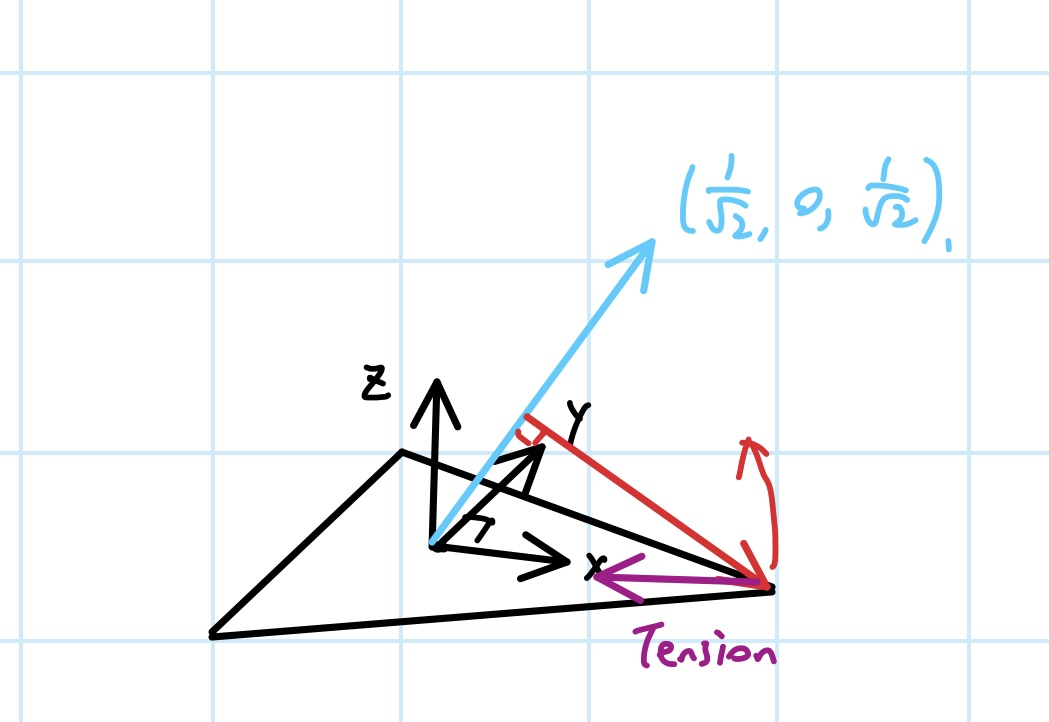
\includegraphics[width=80mm]{phys103_q2d.jpg}
        \caption{Demonstration of the Axis of Rotation}
    \end{center}
\end{figure}

Physically, consider the above image, we can see that the normal vector of the triangle's surface after rotating, its angle with all the standard basis vectors $\hat{x},\hat{y},\hat{z}$ would all change, showing that the mass distribution with respect to each axis starts to change, hence changing the whole inertia tensor. 

On the other hand, when rotating around the axis that aligns with the initial angular velocity, we can see that many parts of the triangle are not orthogonal to the axis (i.e. when having an orthogonal displacement from the axis to the point, there's no material in between). So, the tension force from other parts of the triangle to not align with the cenripetal force needed for this rigid body motion, hence it provides acceleration on the points toward some other directions. These acceleration forces the object to transform into other states, and such transformation forces the direction of rotation to change also, which changes the angular velocity.

\break

\section*{3}
\begin{question}\label{q3}
    A rigid body has principal moments of inertia $I_{xx}=I_0/3$, $I_{yy}=I_{zz}=2I_0/3$.
    \begin{itemize}
        \item[(a)] Find all elements of the moment of the inertia tensor in a reference frame that has been rotated by $\pi/6$ around the $z$ axis counterclockwise.
        \item[(b)] In this new frame, the inertia tensor can be written as a $3\times 3$ matrix with all nine entries. Pretending you do not already know the answer, diagonalize this matrix to find the principal moments of inertia. 
    \end{itemize}
\end{question}

\textbf{Pf:}
\subsection*{(a)}
From the description, the inertia tensor in standard basis is provided as:
\begin{align}
    I = \begin{pmatrix}
        I_{xx}&0&0\\
        0&I_{yy}&0\\
        0&0&I_{zz}
    \end{pmatrix} = \frac{I_0}{3}\begin{pmatrix}
        1&0&0\\
        0&2&0\\
        0&0&2
    \end{pmatrix}
\end{align}
Given a reference frame with rotation of $\frac{\pi}{6}$ around $z$-axis, the rotation matrix (passive rotation) is given as follow:
\begin{align}
    R = \begin{pmatrix}
        \cos(\pi/6)&-\sin(\pi/6)&0\\
        \sin(\pi/6)&\cos(\pi/6)&0\\
        0&0&1
    \end{pmatrix} = \begin{pmatrix}
        \sqrt{3}/2 & -1/2&0\\
        1/2&\sqrt{3}/2&0\\
        0&0&1
    \end{pmatrix}
\end{align}
Then, in the rotated frame (denoted with subscript $1$), the inertia tensor is:
\begin{align}
    I_1 = RIR^T = \frac{I_0}{3}\begin{pmatrix}
        \sqrt{3}/2 & -1/2&0\\
        1/2&\sqrt{3}/2&0\\
        0&0&1
    \end{pmatrix}\begin{pmatrix}
        1&0&0\\0&2&0\\0&0&2
    \end{pmatrix}\begin{pmatrix}
        \sqrt{3}/2 & 1/2&0\\
        -1/2&\sqrt{3}/2&0\\
        0&0&1
    \end{pmatrix} = \frac{I_0}{3}\begin{pmatrix}
        \frac{5}{4} & -\frac{\sqrt{3}}{4} & 0\\
        -\frac{\sqrt{3}}{4} & \frac{7}{4}&0\\
        0&0&2
    \end{pmatrix}
\end{align}
\subsection*{(b)}
To diagonalize the matrix, first consider its characteristic polynomial:
\begin{align}
    \det(I_1-\lambda \Id) &= \det\begin{pmatrix}
        (5I_0/12-\lambda)&-\sqrt{3}I_0/12&0\\
        -\sqrt{3}I_0/12&(7I_0/12-\lambda)&0\\
        0&0&(2I_0/3-\lambda) 
    \end{pmatrix}\\
    &= \paran*{\frac{2I_0}{3}-\lambda}\paran*{\paran*{\frac{5I_0}{12}-\lambda}\paran*{\frac{7I_0}{12}-\lambda}-\frac{I_0^2}{48}}\\
    &= -\paran*{\lambda-\frac{2I_0}{3}}\paran*{\lambda^2-I_0\lambda+\frac{2I_0^2}{9}}\\
    &= -\paran*{\lambda-\frac{2I_0}{3}}^2\paran*{\lambda-\frac{I_0}{3}}
\end{align}
Hence, with $\det(I_1-\lambda\Id)=0$, we get eigenvalues $\lambda=\frac{2I_0}{3},\frac{I_0}{3}$.
\begin{itemize}
    \item First, for $\lambda=\frac{2I_0}{3}$, plug into the equation, we get:
    \begin{align}
        I_1-\frac{2I_0}{3}\Id = \begin{pmatrix}
            -\frac{I_0}{4}& -\frac{\sqrt{3}I_0}{12} & 0\\
            -\frac{\sqrt{3}I_0}{12} & -\frac{I_0}{12}& 0\\
            0&0&0
        \end{pmatrix} = -\frac{I_0}{12}\begin{pmatrix}
            3&\sqrt{3}&0\\
            \sqrt{3}&1&0\\
            0&0&0
        \end{pmatrix}
    \end{align}
    Which, if for vector $\bv=(x,y,z)$, $(I_1-\frac{2I_0}{3}\Id)\bv = \bzero$, we get:
    \begin{align}
        \begin{pmatrix}
            3&\sqrt{3}&0\\
            \sqrt{3}&1&0\\
            0&0&0
        \end{pmatrix}\begin{pmatrix}
            x\\y\\z
        \end{pmatrix}=\bzero \implies \begin{pmatrix}
            \sqrt{3}(\sqrt{3}x+y)\\ \sqrt{3}x+y\\ 0
        \end{pmatrix} = \bzero \implies \sqrt{3}x+y=0,\ z\in\RR
    \end{align}
    \begin{align}
        \implies \bv = \begin{pmatrix}
            x\\y\\z
        \end{pmatrix} = \begin{pmatrix}
            1\\-\sqrt{3}\\0
        \end{pmatrix}x+\begin{pmatrix}
            0\\0\\1
        \end{pmatrix}z = \begin{pmatrix}
            -\frac{1}{2}\\\frac{\sqrt{3}}{2}\\0
        \end{pmatrix}x_1 + \begin{pmatrix}
            0\\0\\1
        \end{pmatrix}z
    \end{align}
    Which, the vector $\bv \in \textmd{span}\{(0,0,1),(-\frac{1}{2},\frac{\sqrt{3}}{2},0)\}$, and they are linearly independent. These are unit eigenvectors associated with $\lambda=\frac{2I_0}{3}$.
    \item Then, for $\lambda=\frac{I_0}{3}$, plug into the equation, we get:
    \begin{align}
        I_1-\frac{I_0}{3}\Id = \begin{pmatrix}
            \frac{I_0}{12}&-\frac{\sqrt{3}I_0}{12}&0\\
            -\frac{\sqrt{3}I_0}{12}&\frac{I_0}{4}&0\\
            0&0&\frac{I_0}{3}
        \end{pmatrix}=\frac{I_0}{12}\begin{pmatrix}
            1&-\sqrt{3}&0\\
            -\sqrt{3}&3&0\\
            0&0&4
        \end{pmatrix}
    \end{align}
    Which, if for vector $\bv = (x,y,z)$, $(I_1-\frac{I_0}{3}\Id)\bv=\bzero$, we get:
    \begin{align}
        \begin{pmatrix}
            1&-\sqrt{3}&0\\
            -\sqrt{3}&3&0\\
            0&0&4
        \end{pmatrix}\begin{pmatrix}
            x\\y\\z
        \end{pmatrix} = \bzero \implies \begin{pmatrix}
            x-\sqrt{3}y\\ \sqrt{3}(x-\sqrt{3}y)\\ 4z
        \end{pmatrix}=\bzero\implies z=0,\ x-\sqrt{3}y=0
    \end{align}
    \begin{align}
        \implies \bv=\begin{pmatrix}
            x\\y\\z
        \end{pmatrix}=\begin{pmatrix}
            \sqrt{3}\\1\\0
        \end{pmatrix}y = \begin{pmatrix}
            \frac{\sqrt{3}}{2}\\\frac{1}{2}\\0
        \end{pmatrix}y_1
    \end{align}
    So, $\bv\in \textmd{span}\{(\frac{\sqrt{3}}{2},\frac{1}{2},0)\}$, this is a unite eigenvector associated with $\lambda = \frac{I_0}{3}$.
\end{itemize}
Now, if chosen the set of eigenvectors as $\be_1 = (\frac{\sqrt{3}}{2},\frac{1}{2},0)$, $\be_2=(-\frac{1}{2},\frac{\sqrt{3}}{2},0)$, and $\be_3 = (0,0,1)$, one can check that they're mutually orthogonal (i.e. $\be_i \cdot \be_j = 0$, and $\|\be_i\|=1$ for all index $i\neq j$). Hence, it is an orthonormal basis (which consists of eigenvectors of $I_1$, corresponding to $\lambda=\frac{I_0}{3},\frac{2I_0}{3},\frac{2I_0}{3}$ respectively). Then, let the diagonal matrix $D$, and change of basis matrix $U$ (which is also a special orthogonal matrix) be as follow:
\begin{align}
    &D=\begin{pmatrix}
        \frac{I_0}{3}&0&0\\
        0&\frac{2I_0}{3}&0\\
        0&0&\frac{2I_0}{3}
    \end{pmatrix}, \quad U = \begin{pmatrix}
        | & |&|\\
        \be_1&\be_2&\be_3\\
        |&|&|
    \end{pmatrix} = \begin{pmatrix}
        \frac{\sqrt{3}}{2}&-\frac{1}{2}&0\\
        \frac{1}{2}&\frac{\sqrt{3}}{2}&0\\
        0&0&1
    \end{pmatrix}, \ U^{-1}=U^T
\end{align}
(Note: For special orthogonal matrix, or column vectors form an orthonormal basis, $UU^T = U^TU = \Id$). 

Then, after diagonalization, we get:
\begin{align}
    I_1 = U^{-1}DU = \begin{pmatrix}
        \frac{\sqrt{3}}{2}&\frac{1}{2}&0\\
        -\frac{1}{2}&\frac{\sqrt{3}}{2}&0\\
        0&0&1
    \end{pmatrix}\begin{pmatrix}
        \frac{I_0}{3}&0&0\\
        0&\frac{2I_0}{3}&0\\
        0&0&\frac{2I_0}{3}
    \end{pmatrix}\begin{pmatrix}
        \frac{\sqrt{3}}{2}&-\frac{1}{2}&0\\
        \frac{1}{2}&\frac{\sqrt{3}}{2}&0\\
        0&0&1
    \end{pmatrix}
\end{align}
Which, $D=I$, the original inertia tensor.

\break

\section*{4}
\begin{question}\label{q4}
    A rigid body has an axis of symmetry, which we shall designate axis $1$. The principal moment of inertia about this axis is $I_1$, while the principal moments of inertia about the remaining two principal axes are $I_2=I_3=I_0\neq I_1$. No torques act on the body, and it has some initial angular velocity $(w_1,w_2,w_3)=(w_{1,0},w_{2,0},w_{3,0})$.
    \begin{itemize}
        \item[(a)] Show that the body precesses around axis $1$: $w_1$ is constant and $w_2,w_3$ both oscillate sinusoidally, with the same magnitude and a $\pi/2$ phase difference.
        \item[(b)] Does either the frequency or direction of the precession depend on whether the body is prolate (like a baseball bat) or oblate (like a frisbee)? 
    \end{itemize}
\end{question}

\textbf{Pf:}

We'll assume all vectors are represented under body frame, and initially $\bw_0 = (w_{1,0},w_{2,0},w_{3,0})$ under body frame also (i.e. initially the body frame aligns with standard basis).
\subsection*{(a)}
First, recall that under body frame, Euler's equation is satisfied:
\begin{align}
    \begin{cases}
        I_1\frac{dw_1}{dt}=N_1+(I_2-I_3)w_2w_3\\
        I_2\frac{dw_2}{dt}=N_2+(I_3-I_1)w_3w_1\\
        I_3\frac{dw_3}{dt}=N_3+(I_1-I_2)w_1w_2
    \end{cases}
\end{align}
With torque $\bN=\bzero$ (since assumes no torque is acting on the body), then $N_1=N_2=N_3=0$. Also, plug in $I_2=I_3 = I_0$, we get:
\begin{align}
    \begin{cases}
        I_1\frac{dw_1}{dt}=0\\
        I_0\frac{dw_2}{dt}=(I_0-I_1)w_3w_1\\
        I_0\frac{dw_3}{dt}=-(I_0-I_1)w_1w_2
    \end{cases}
\end{align}
The first equation provides $\frac{dw_1}{dt}=0$, hence $w_1$ is constant; with initial condition $w_1(0)=w_{1,0}$, we get $w_1(t) = w_{1,0}$. Plug this into the other two equations, and take differentiation again, we get:
\begin{align}
    \begin{cases}
        \frac{dw_2}{dt}=\frac{w_{1,0}(I_0-I_1)}{I_0}w_3\\
        \frac{dw_3}{dt}=-\frac{w_{1,0}(I_0-I_1)}{I_0}w_2
    \end{cases}, \quad \begin{cases}
        \frac{d^2w_2}{dt^2} = \frac{w_{1,0}(I_0-I_1)}{I_0}\frac{dw_3}{dt}\\
        \frac{d^2w_3}{dt^2}=-\frac{w_{1,0}(I_0-I_1)}{I_0}\frac{dw_2}{dt}
    \end{cases}\implies \begin{cases}
        \frac{d^2w_2}{dt^2} = -\paran*{\frac{w_{1,0}(I_0-I_1)}{I_0}}^2w_2\\
        \frac{d^2w_3}{dt^2}=-\paran*{\frac{w_{1,0}(I_0-I_1)}{I_0}}^2w_3
    \end{cases}
\end{align}
Which, the above differential equations are simple harmonic oscillators. Let $\Omega := \frac{w_{1,0}(I_0-I_1)}{I_0}$, the solution to $w_2$ is $w_2=A\cos(\Omega t+\phi)$ for some amplitude $A$ and phase $\phi$. Then, if taken a derivative, with the first order differential equations on the left, we get:
\begin{align}
    \Omega w_3 = \frac{dw_2}{dt} = -\Omega A\sin(\Omega t+\phi) = &\Omega A\paran*{\cos(\Omega t+\phi)\cos\paran*{\frac{\pi}{2}}-\sin(\Omega t+\phi)\sin\paran*{\frac{\pi}{2}}} = \Omega A\cos\paran*{\Omega t+\phi + \frac{\pi}{2}}\\
    &\implies w_3 = A\cos\paran*{\Omega t+\phi + \frac{\pi}{2}}
\end{align}
(Note: the second line is true, because by assumption $I_0\neq I_1$, and both are not $0$; if assume $w_{1,0}\neq 0$, we get $\Omega\neq 0$).

So, this proves that under the body frame, $w_2,w_3$ are sinusoidal waves with phase difference of $\frac{\pi}{2}$, while $w_1$ is kept constant. This shows that in the body frame, the angular velocity precesses around axis $1$, so the body precess around axis $1$, regardless of the amplitude $A$.

\subsection*{(b)}
First, about the frequency of precession, with the above formulas, it's given by $\Omega = \frac{w_{1,0}(I_0-I_1)}{I_0}$ (more generally, using $|\Omega|$ is sufficient since frequency doesn't care about the direction of the precession). 
Which, if $I_0$ and $I_1$ are close, we get that $|\Omega|$ is small, hence it takes longer period to complete one precession; else, if $I_0$ and $I_1$ varies a lot, then $|\Omega|$ is also large, hence it'll take shorter period to complete one percession. However, this requires a more precise understanding about the mass distribution, knowing if the object is prolate or oblate is not sufficient to tell (for instance, under fixed $I_0$, take $I_1 = \frac{I_0}{2}<I_0$ and $I_1 = \frac{3I_0}{2}>I_0$ provides the same $|\Omega|=\frac{w_{1,0}}{2}$, while the first situation is close to oblate, and the second situation is close to prolate).

\hfil

Now, about the direction of precession, we care more about the sign of $\Omega$:
\begin{itemize}
    \item If the body is prolate (like a baseball bat), since with respect to axis $1$ (where the bat has rotational symmetry with) the mass distribution is in general closer to the axis, while respect to other two axes the bat has more mass distributed farther from center of mass, then $I_1 < I_0$; which, $\Omega =w_{1,0}(1-\frac{I_1}{I_0})>0$, showing that with respect to the body frame, angular velocity $\bw$ is precessing counterclockwise around axis 1.
    \item If the body is oblate (like a frisbee), then the mass is scattered more outward for axis $1$ compared to the other axes, hence $I_1>I_0$. Which, $\Omega=w_{1,0}(1-\frac{I_1}{I_0})<0$, showing that with respect to the body frame, angular velocity $\bw$ is precessing clockwise around axis 1 instead.
\end{itemize}
Hence, the shape of the object (being prolate or oblate) would affect the direction of the precession, however it's precise effect on the frequency cannot be concluded by the rough shape (requires more knowledge about mass distribution of the object).

\break

\section*{5 (Insert image)}
\begin{question}\label{q5}
    Model a space station as a hollow cylinder of mass $M$, radius $R$, and length $D$; the endcaps are of negligible mass. Initially, the station spins about its symmetry axis (which we'll take to be the $z$-axis) with angular velocity $w_0$.
    \begin{itemize}
        \item[(a)] Find its inertia tensor about its center.
        \item[(b)] A meteor of mass $m$ and velocity $v_0$, moving in the $x$ direction, strikes the station very near one of the endcaps and bounces directly back with velocity $-v_0/2$. Find the station's CM velocity and angular momentum after the collision.
        \item[(c)] Show that the station wobbles (i.e. the direction of the angular velocity rotates). Find the period of the wobble, as experienced by a person on the station.  
    \end{itemize}
\end{question}

\textbf{Pf:}
\subsection*{(a)}
Again, since assuming it has no width directly is going to cause some calculation problem, so we'll assume the thickness of the cylinder is $\epsilon>0$, and at the end take the limit $\epsilon\rightarrow 0$. Now, suppose the inner radius is $R-\frac{\epsilon}{2}$ and outer radius is $R+\frac{\epsilon}{2}$, we get that the total volume of the (almost) hollow cylinder is $V=D\pi((R+\frac{\epsilon}{2})^2-(R-\frac{\epsilon}{2})^2) = \pi D2R\epsilon$. So, the density $\rho = \frac{M}{V}=\frac{M}{2\pi RD\epsilon}$.

Since the center of mass of the cylinder is precisely at half of the height, then in cylindrical coordinates, $z\in [-\frac{D}{2},\frac{D}{2}]$, angle $\theta\in [0,2\pi]$, and $r\in [R-\frac{\epsilon}{2},R+\frac{\epsilon}{2}]$. So, the inertia tensor about its center is given as follow:
\begin{align}
    I(\epsilon) = \int_V \begin{pmatrix}
        y^2+z^2 & -xy & -xz\\
        -xy & x^2+z^2 & -yz\\
        -xz & -yz & x^2+y^2
    \end{pmatrix}\rho dV
\end{align}
Based on the symmetry on $x$ and $y$, if using the standard cartesian coordinate for integration, the bound of $x,y,z$ are all in the form  of finite sums from $-a$ to $a$. Hence, if integrate $xy,xz,yz$, we all get $0$ (for $xy,yz$, if integrate $y$ first, since it's an odd function of $y$, the integral provides $0$; for $z$, since separating out variable $z$ individually to integrate from $-\frac{D}{2}$ to $\frac{D}{2}$ provides $0$, the total integral is again $0$). Then, we only need to consider the diagonals. In this case, we'll use cylindrical coordinate, and we get the following:
\begin{align}
    X &:= \int_{z=-\frac{D}{2}}^{\frac{D}{2}}\int_{r=R-\frac{\epsilon}{2}}^{R+\frac{\epsilon}{2}}\int_{\theta =0}^{2\pi}x^2 r\ d\theta\ dr\ dz = \int_{z=-\frac{D}{2}}^{\frac{D}{2}}\int_{r=R-\frac{\epsilon}{2}}^{R+\frac{\epsilon}{2}}\int_{\theta =0}^{2\pi}r^3\cos^2(\theta)\ d\theta\ dr\ dz\\
    &= \pi D\cdot\frac{1}{4}r^4\bigg|_{R-\frac{\epsilon}{2}}^{R+\frac{\epsilon}{2}} = \frac{\pi DR\epsilon}{2}\paran*{R^2+\frac{\epsilon^2}{4}}
\end{align}
\begin{align}
    Y &:=\int_{z=-\frac{D}{2}}^{\frac{D}{2}}\int_{r=R-\frac{\epsilon}{2}}^{R+\frac{\epsilon}{2}}\int_{\theta =0}^{2\pi}y^2 r\ d\theta\ dr\ dz = \int_{z=-\frac{D}{2}}^{\frac{D}{2}}\int_{r=R-\frac{\epsilon}{2}}^{R+\frac{\epsilon}{2}}\int_{\theta =0}^{2\pi}r^3\sin^2(\theta)\ d\theta\ dr\ dz\\
    &= \pi D\cdot\frac{1}{4}r^4\bigg|_{R-\frac{\epsilon}{2}}^{R+\frac{\epsilon}{2}} = \frac{\pi DR\epsilon}{2}\paran*{R^2+\frac{\epsilon^2}{4}} = X
\end{align}
\begin{align}
    Z &:=\int_{z=-\frac{D}{2}}^{\frac{D}{2}}\int_{r=R-\frac{\epsilon}{2}}^{R+\frac{\epsilon}{2}}\int_{\theta =0}^{2\pi}z^2 r\ d\theta\ dr\ dz = \int_{z=-\frac{D}{2}}^{\frac{D}{2}}z^2dz\int_{r=R-\frac{\epsilon}{2}}^{R+\frac{\epsilon}{2}}rdr\int_{\theta=0}^{2\pi}d\theta\\
    &= 2\pi\paran*{\frac{1}{2}r^2\bigg|_{R-\frac{\epsilon}{2}}^{R+\frac{\epsilon}{2}}}\paran*{\frac{1}{3}z^3\bigg|_{-\frac{D}{2}}^{\frac{D}{2}}} = \frac{\pi D^3R\epsilon}{6}
\end{align}
(Note: $\int_{0}^{2\pi}\cos^2(\theta)d\theta=\int_{0}^{2\pi}\sin^2(\theta)d\theta=\pi$).

Then, the inertia tensor of the center becomes:
\begin{align}
    I(\epsilon)=\rho\begin{pmatrix}
        Y+Z&0&0\\
        0&X+Z&0\\
        0&0&X+Y
    \end{pmatrix}=\rho\begin{pmatrix}
        X+Z&0&0\\
        0&X+Z&0\\
        0&0&2X
    \end{pmatrix}
\end{align}
Which, take the limit $\epsilon\rightarrow 0$, we get:
\begin{align}
    \lim_{\epsilon\rightarrow 0}\rho X=\lim_{\epsilon\rightarrow 0}\frac{M}{2\pi RD\epsilon}\cdot \frac{\pi DR\epsilon}{2}\paran*{R^2+\frac{\epsilon^2}{4}}=\frac{MR^2}{4},\quad \lim_{\epsilon\rightarrow 0}\rho Z=\lim_{\epsilon\rightarrow 0}\frac{M}{2\pi RD\epsilon}\cdot\frac{\pi D^3R\epsilon}{6}=\frac{MD^2}{12}
\end{align}
Hence, the inertia tensor of the center is given by:
\begin{align}
    I = \lim_{\epsilon\rightarrow 0}I(\epsilon) = \begin{pmatrix}
        \paran*{\frac{MR^2}{4}+\frac{MD^2}{12}}&0&0\\
        0&\paran*{\frac{MR^2}{4}+\frac{MD^2}{12}}&0\\
        0&0& \frac{MR^2}{2}
    \end{pmatrix}
\end{align}

\subsection*{(b)}
\begin{figure}[h!]
    \begin{center}
        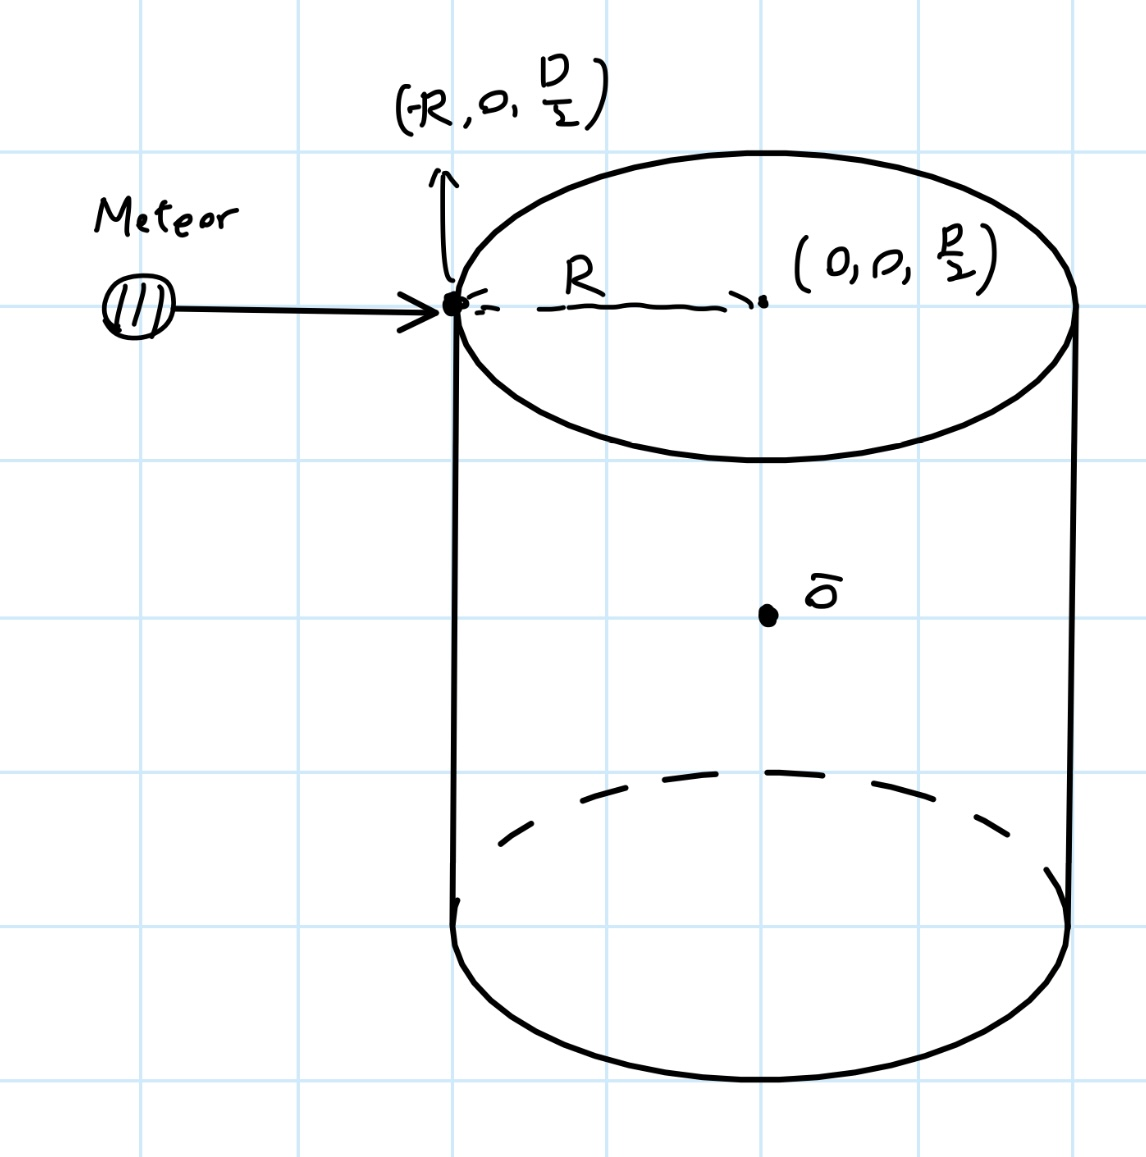
\includegraphics[width=70mm]{phys103_q5b.jpg}
        \caption{Setup for the collision}
    \end{center}
\end{figure}

First, if consider the system's linear momentum, if assume initially the station is not moving in the observer's frame, then the momentum initially would all be provided by the meteor, so $\bP_0 = mv_0\hat{x}$ (since the initial speed of the meteor is $v_0$ in $x$-direction).

Then, since the meteor bounces back with velocity $-\frac{v_0}{2}$ (still in $x$-direction), then the final momentum of the meteor $\bP_m = -\frac{mv_0}{2}\hat{x}$. By conservation of linear momentum, the final momentum of the station, $\bP_s$ must satisfy $\bP_s + \bP_m = \bP_f = \bP_0$, then $\bP_s = \bP_0-\bP_m = mv_0\hat{x}-(-\frac{mv_0}{2})\hat{x} = \frac{3mv_0}{2}\hat{x}$. Becacuse $\bP_s= M\bv_{\textmd{CM}}$ (where $\bv_{\textmd{CM}}$ denotes the velocity of the CM of the station), then $M\bv_{\textmd{CM}} = \frac{3mv_0}{2}\hat{x}$, so $\bv_{\textmd{CM}} = \frac{3mv_0}{2M}\hat{x}$.

\hfil

Now, to consider the angular momentum, WLOG, we'll assume the meteor collides on the upper part, which because it bounces directly back of its original direction, then the surface it collides must be orthogonal to its initial motion, hence it must happen when $y=0$; and since it's assumed to collide near the end (and because the meteor is initially heading toward positive $x$-direction), then the meteor collides with the station at location $\br_0=(-R, 0, \frac{D}{2})$ (based on the graph). Which, right before the collision, since the meteor has linear momentum $\bP_0 = mv_0\hat{x}$, then its initial angular momentum of the meteor $\bL_{0,m} = \br_0\times \bP_0 = \frac{mv_0D}{2}\hat{y}$.

Also, initially the station was rotating around $z$-axis with angular velocity $w_0$, its initial angular velocity is $w_0\hat{z}$. Hence, the station's initial angular momentum $\bL_{0,s}$ is given by:
\begin{align}
    \bL_{0,s}=I(w_0\hat{z}) = \begin{pmatrix}
        \paran*{\frac{MR^2}{4}+\frac{MD^2}{12}}&0&0\\
        0&\paran*{\frac{MR^2}{4}+\frac{MD^2}{12}}&0\\
        0&0& \frac{MR^2}{2}
    \end{pmatrix}\begin{pmatrix}
        0\\0\\w_0
    \end{pmatrix} = \frac{MR^2w_0}{2}\hat{z}
\end{align}
Hence, the total initial angular momentum is $\bL_0 = \bL_{0,m}+\bL_{0,s} = (0,\frac{mv_0D}{2},\frac{MR^2w_0}{2})$.

Which, right after the impact, the linear momentum of the meteor $\bP_m = -\frac{mv_0}{2}\hat{x}$, hence the meteor's angular momentum right after the impact is $\bL_m = \br_0\times \bP_m = -\frac{mv_0D}{4}\hat{y}$. Finally, based on conservation of angular momentum, the station's final angular momentum $\bL_s$ (after the collision) must satisfy $\bL_s+\bL_m=\bL_0$, showing that $\bL_s = \bL_0-\bL_m = (0,\frac{mv_0D}{2}, \frac{MR^2w_0}{2})-(0,-\frac{mv_0D}{4},0) = (0,\frac{3mv_0D}{4},\frac{MR^2w_0}{2})$. 

(Note: Since the CM velocity of the station is solely in $\hat{x}$-direction, while the station starts moving from the origin, then its position is solely radial in $\hat{x}$-direction, showing that it has no orbital angular momentum. The above angular momentum $\bL_s$ is solely the spin angular momentum of the station after the collision, which can be used directly in part (c)).

\subsection*{(c)}
If we view in body frame (which aligns with the frame of standard basis right after the collision), then we get the following for the initial angular velocity $\bw_i$ right after the collision:
\begin{align}
    \bL_s = I\bw_i \implies \bw_i &= I^{-1}\bL_s = \begin{pmatrix}
        \frac{12}{3MR^2+MD^2}&0&0\\
        0&\frac{12}{3MR^2+MD^2}&0\\
        0&0&\frac{2}{MR^2}
    \end{pmatrix}\begin{pmatrix}
        0\\\frac{3mv_0D}{4}\\\frac{MR^2w_0}{2}
    \end{pmatrix} = \begin{pmatrix}
        0\\ \frac{9mv_0D}{3MR^2+MD^2}\\ w_0
    \end{pmatrix}
\end{align}
Which, assume after the angular momentum has changed, there is no torque applied on the station, then using Euler's Equation (like in Question \ref{q4}), we get:
\begin{align}
    \begin{cases}
        I_1\frac{dw_1}{dt}=N_1+(I_2-I_3)w_2w_3\\
        I_2\frac{dw_2}{dt}=N_2+(I_3-I_1)w_3w_1\\
        I_3\frac{dw_3}{dt}=N_3+(I_1-I_2)w_1w_2
    \end{cases}, \quad N_1=N_2=N_3=0,\ I_1=I_2 = \frac{MR^2}{4}+\frac{MD^2}{12},\ I_3 = \frac{MR^2}{2}
\end{align}
\begin{align}
    \implies \begin{cases}
        \frac{dw_1}{dt}=\frac{(I_1-I_3)}{I_1}w_2w_3\\
        \frac{dw_2}{dt}=-\frac{(I_1-I_3)}{I_1}w_3w_1\\
        \frac{dw_3}{dt}=0
    \end{cases}
\end{align}
The third equation implies that $w_3$ is constant, hence with $w_3(0)=w_0$ given in (63), $w_3(t)=w_0$. Plug into the other two equations, we get:
\begin{align}
    \begin{cases}
        \frac{dw_1}{dt}=\frac{w_0(I_1-I_3)}{I_1}w_2\\
        \frac{dw_2}{dt}=-\frac{w_0(I_1-I_3)}{I_1}w_1
    \end{cases} \implies \Omega := \frac{w_0(I_1-I_3)}{I_1},\ \begin{cases}
        \frac{dw_1}{dt}=\Omega w_2\\
        \frac{dw_2}{dt}=-\Omega w_1
    \end{cases}\implies \begin{cases}
        \frac{d^2w_1}{dt^2}=\Omega \frac{dw_2}{dt} = -\Omega^2 w_1\\
        \frac{d^2w_2}{dt^2}=-\Omega \frac{dw_1}{dt} = -\Omega^2 w_2
    \end{cases}
\end{align}
Based on the solution provided in Question \ref{q4}, we know $w_1 = A\cos(\Omega t+\phi),\ w_2=A\cos(\Omega t+\phi+\frac{\pi}{2})$ for some amplitude $A$ and phase $\phi$. With the given initial condition, we know $w_2(0)=A\cos(\phi+\frac{\pi}{2}) = -A\sin(\phi) =\frac{9mv_0D}{3MR^2+MD^2}\neq 0$, which shows $A\neq 0$, so the angular momentum is not fixed when viewed in the body frame. Hence, with $w_1,w_2$ being sinusoidal waves of frequency $\Omega$, this shows that the station is in fact wobbling, and with frequency $\Omega$.

Finally, since $\Omega = \frac{w_0(I_1-I_3)}{I_1}$, we get the following for the frequency (up to a sign difference):
\begin{align}
    \Omega &= w_0\cdot \paran*{\frac{MD^2}{12}+\frac{MR^2}{4}-\frac{MR^2}{2}}\cdot\frac{12}{3MR^2+MD^2} = w_0\cdot\frac{MD^2-3MR^2}{12}\cdot \frac{12}{MD^2+3MR^2} \\
    &= w_0\cdot\frac{MD^2-3MR^2}{MD^2+3MR^2} = w_0\cdot\frac{D^2-3R^2}{D^2+3R^2}
\end{align}

%test change
\end{document}